\chapter{Evaluation}

The following chapter describes the evaluation and introduces the results from the testing of the prototype. 

There were conducted two tests, an internal and a user test. This was done to test whether the prototype was functional on a technical level and to test whether is was usable by people not part of this project. 


\section{Internal Test}

To test the accuracy of the prototype, an internal test was carried out. The following hypotheses have been stated for the internal test: \\

H\textsubscript{0}: The prototype works less than 90\% of the time.\\

H\textsubscript{A}: The prototype works more than or equal to 90\% of the time.\\

The test consisted of the copper plates being connected 25 times each. First the index finger were tested with the thumb afterwards the middle finger with the thumb. Whenever the yellow light on the system lit up it was considered a success. If the light did not turn on it was considered a failure. The times it succeeded and failed were counted.\\

The results ended up being as follows:

\begin{itemize}
\item Index finger connection test: 23 out of 25. 
\item Middle finger connection test: 25 out of 25.\\
\end{itemize}


The results have been analysed statistically using R\citep{R}. R is a language used for statistical analysis. All the statistics have been calculated with a probability of success, p, of 0.5.\\
The results from the index finger connection test showed a p-value of:

\begin{equation}
	1.943*10^{-5}
\end{equation} 

Whenever the p-value is less than the 0.05 significance level, a conclusion can be drawn from the test. In this case the H\textsubscript{0} is rejected for the index finger, since the test gave a probability of success of 0.92(92\%).
prototype worked at least 90\% of the time when connecting the index finger and thumb. \\

The results for the middle finger connection test showed a p-value of:

\begin{equation}\label{Pval2}
	5.96*10^{-8}
\end{equation} 

The p-value lies below the 0.05 significance level, so a conclusion can be made. This means that this connection works at least 90\% of the time, and the H\textsubscript{0} is rejected for the middle finger also. \\

Another internal test was carried out to test the accuracy of the effects. The test was conducted in a similar way, the effects were applied and then used. 
As long as the effect worked and changed the voice input, it was considered a success. \\

In the first test, the system worked 18 out of 25 times for both gestures.
Since the gesture effects showed the same results, the p-value is the same for both gestures. 
The p-value ended up being 0.04329 which is lower than the 0.05 significance level and therefore the result can be concluded upon. Thus, the H\textsubscript{0} is accepted, since the prototype worked less than 90\% of the time with the gestures. \\

During the first tests, the system had a loose wire. The issue was fixed and the tests were then conducted once again with much better results:

All the tests worked 25 out of 25 times. \\

This gave a p-value equal to equation \ref{Pval2}, which is much less than the 0.05 significance level and a probability of success equal to 1(100\%) and therefore H\textsubscript{0} are rejected for all the tests.

\section{User Test}
When conducting this user test, it was the intention to get some data from the users about the different effects and gestures. 

\subsection{Evaluation Plan}
To evaluate the working prototype three hypotheses based on the device were stated. They are as follows:

\begin{enumerate}
\item Participants understand the link between gesture and effect
\item The design is awkward to wear
\item The participants will have no clear preference of effect
\end{enumerate} 

To evaluate the hypotheses a test was conducted with the goal to either prove or disprove them. First the participants were asked to sign a consent form which together with the script can be found here: Appendix \ref{Consent} and \ref{Script}. The test then consisted of the participants doing different tasks, which was followed by a few questions to determine whether to prove or disprove the hypotheses. The results of those questions can be found in \ref{ch:appB} The questions can be found her Appendix \ref{Questionnaire}. 

\subsection{Apparatus and Setup}

The following equipment was used to perform the test:
\begin{itemize}
 \item Two laptops
 \item Zoom H4N microphone 
 \item Headphones
 \item The Prototype
\end{itemize}

The following figure \ref{Setup} shows the setup of the evaluation. One person wearing the system, a facilitator, and one person that makes sure the system works and has the microphone in 
his left hand (technician).

\begin{minipage}{\linewidth}% to keep image and caption on one page
\makebox[\linewidth]{%        to center the image
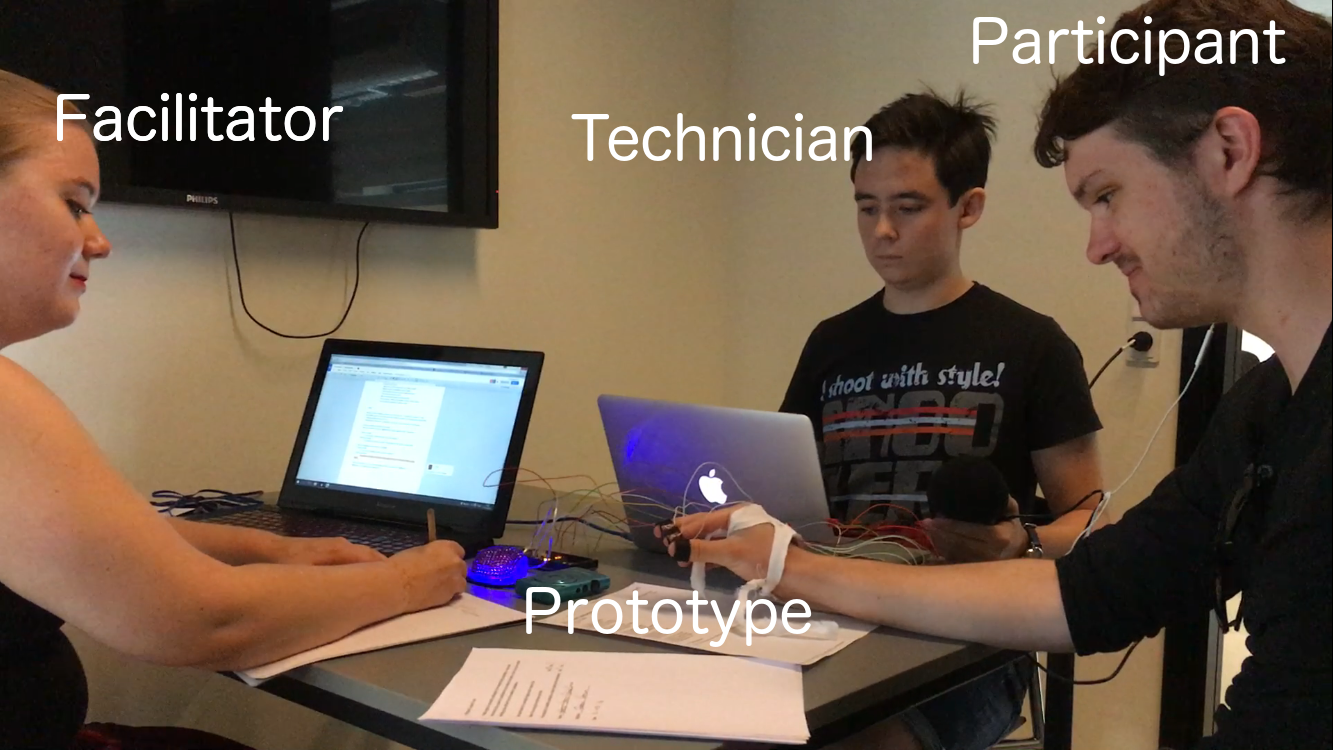
\includegraphics[keepaspectratio=true,scale=0.4]{Setup}}
\captionof{figure}{The Test Setup. There is a facilitator, a technician, and a participants. The technician has the microphone in his left hand.}\label{Setup}
\end{minipage}\\

\subsection{Results}
The hypotheses previously stated will be rejected or kept based on the results from the questions asked during the interview.

The first hypothesis deals with the link between the gesture and the effect. Here the question were asked: Did the gesture makes sense together with the effect? All the participants answered yes to this and also said why it was. A female participant said “[it is] like turning a button up and down”. A male participant mentioned that “It is like turning [the volume] up and down”. Another male participant said “[it is] like turning a knob”. These three are examples of the exact idea the gesture was based upon.\\ 

The second hypothesis deals with the physical aspects of the prototype. Here the question asked was: Was the device comfortable to wear? Again all participants agreed. The device was comfortable to wear. \\

The third hypothesis deals with preference of effect. The participants were asked: Which effect did you prefer? All participants, except one, answered pitch-shifting. This presents a clear preference for the pitch-shifting effect. \\

Aside from what the quantitative data from the questions, there were some additional data. Mainly the comments and feedback from the participants during the test which is analysed as qualitative data. Especially the participant with a musical background gave a lot of useful feedback regarding the prototype. Four out of the ten participants stated that they could not hear a difference between the major and minor harmonics. The participant with a musical background heard the difference clearly. However an assumption could then be made that the other participants could not hear the difference since they did not know what they were listening for. \\

They could all clearly hear the difference between shifting the pitch up or down. However five participants mentioned that the pitch-shifting is very sensitive and that there is not a lot of middle ground between no effect and full effect. \\

Another thing mentioned by three of the participants is that even though all participants found the gestures intuitive, holding them for longer periods of time could be very straining and cramp-inducing on their hand. \\

When asked whether they thought the prototype useful or not, nine of the ten participants said that they thought it could be. Some said that it could be useful in theatre performance and another said that it gives more control to the singer. Both of these are some of the ideas this project is based on. \\

The one participant we had who had a musical background also gave some additional constructive feedback. She stated that the harmonise effect lacks the ability to be able to choose the intervals you want. She said that it would be "incredibly smart if the first notes added the 3rd interval and then the 5th interval, and maybe even removed the 3rd interval if you twisted the wrist even further. Then you are in more control of the notes and the expression the music makes." Changing the intervals is something to consider for further iterations. 

\section{Discussion}
Several parameters of these tests must be considered before any conclusions are drawn. Only one participant from this user test fits this project's target group. This does affect the results quite a bit since participants of this test  do not have the necessary knowledge to know how the prototype could be utilised, and therefore cannot give very useful feedback on the musical aspect of the prototype.
Then there is the issue that the first half of the participants tested a prototype with a loose wire which made it act oddly and made it more prone to not react to the gestures made by the participant. The questions were also mostly yes/no questions which gives a rather limited view of the participants' reactions and views of the prototype. A Likert scale would maybe have been more appropriate for more nuanced answers.

\section{Conclusion}
Based on the results from these two tests it can be concluded that the technical parts of the prototype works as intended. Even though the system is simple, it works every time and all the participants like the concept and thought it useful, even though they may not have correct knowledge to deem it so. Using the feedback that was gathered, certain adjustments could be implemented, ie. less sensitivity to the pitch-shifting and more adjustability to the harmoniser. The concept of the prototype working with the hands works very well although further exploration of different gestures and effects could be a good idea. 


